\section{Features and Interaction Design}
\label{implementation}


\begin{wrapfigure}{O}{0.3\textwidth}
  \centering
  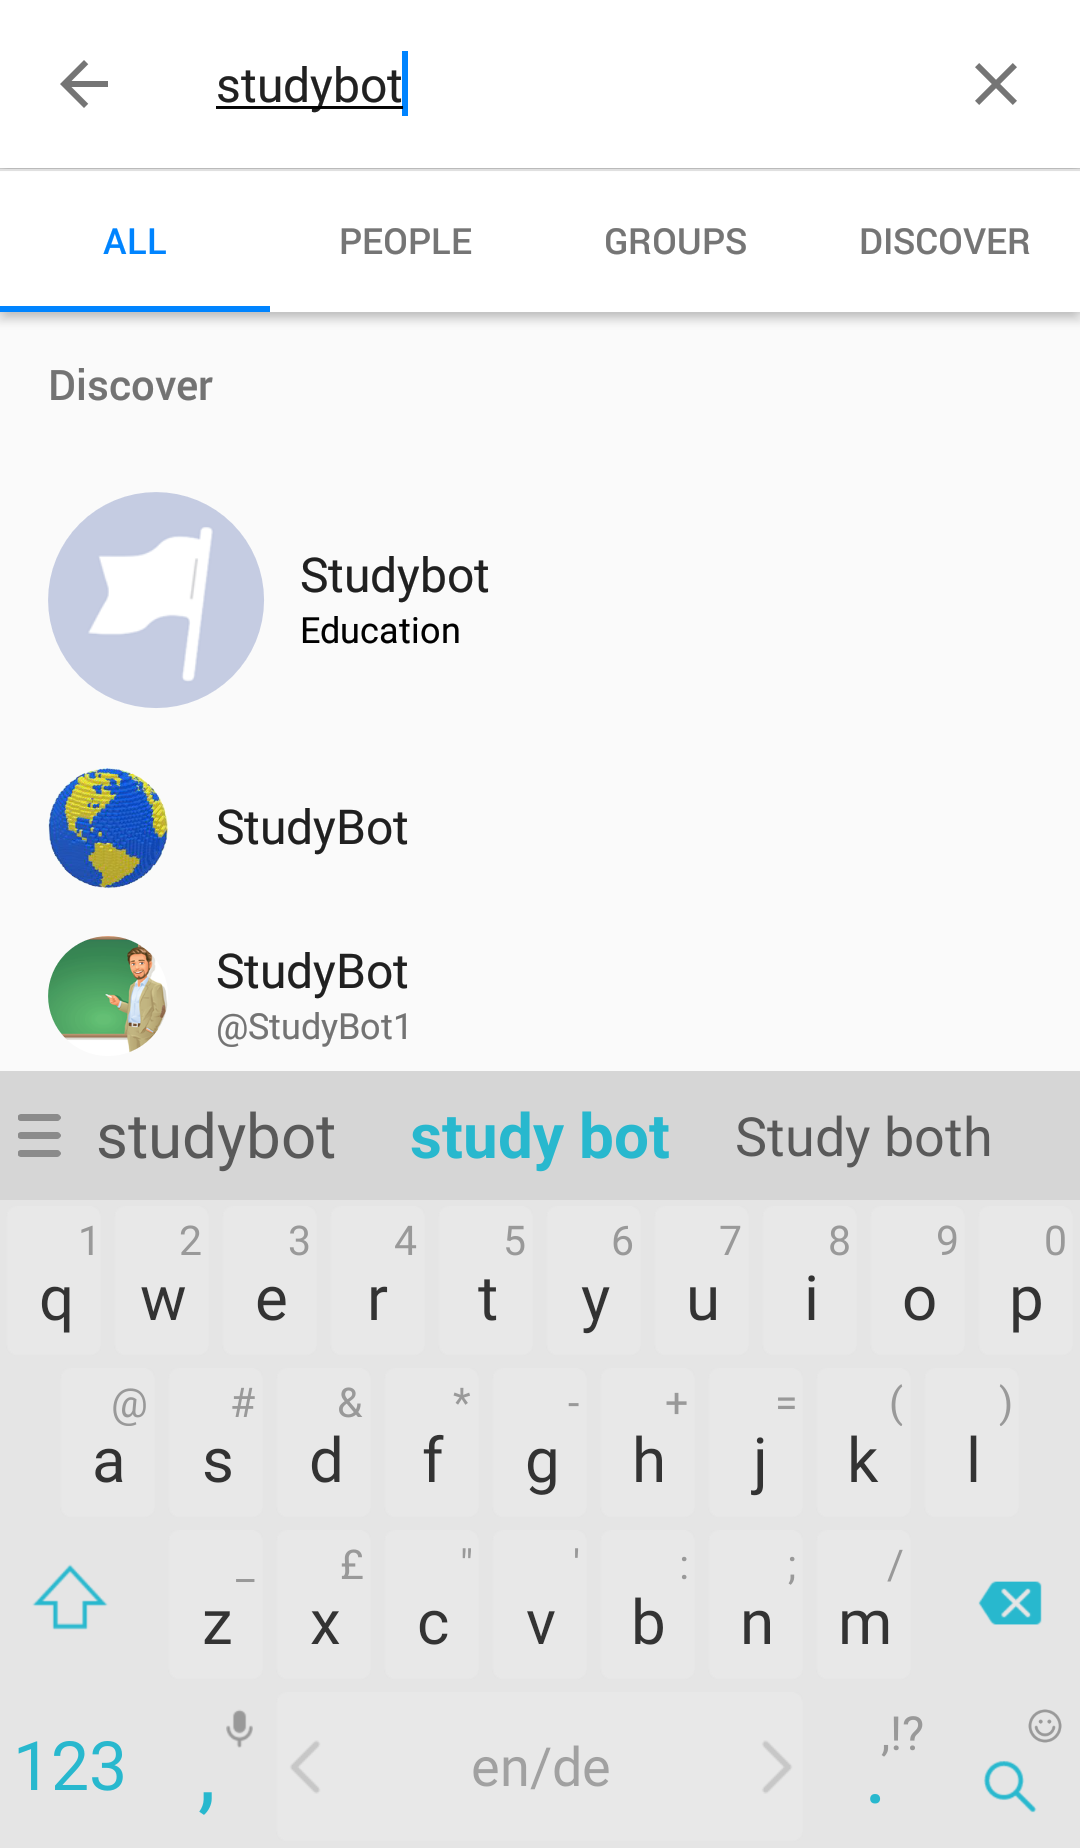
\includegraphics[width=0.28\textwidth]{images/interface/01-search.png}
	\caption{Search}
	\label{fig:01-search}
\end{wrapfigure}

At this point it is defined what the example chatbot should be able to do,
and which technologies are used for its implementation.
\\

\begin{wrapfigure}{O}{0.3\textwidth}
  \centering
  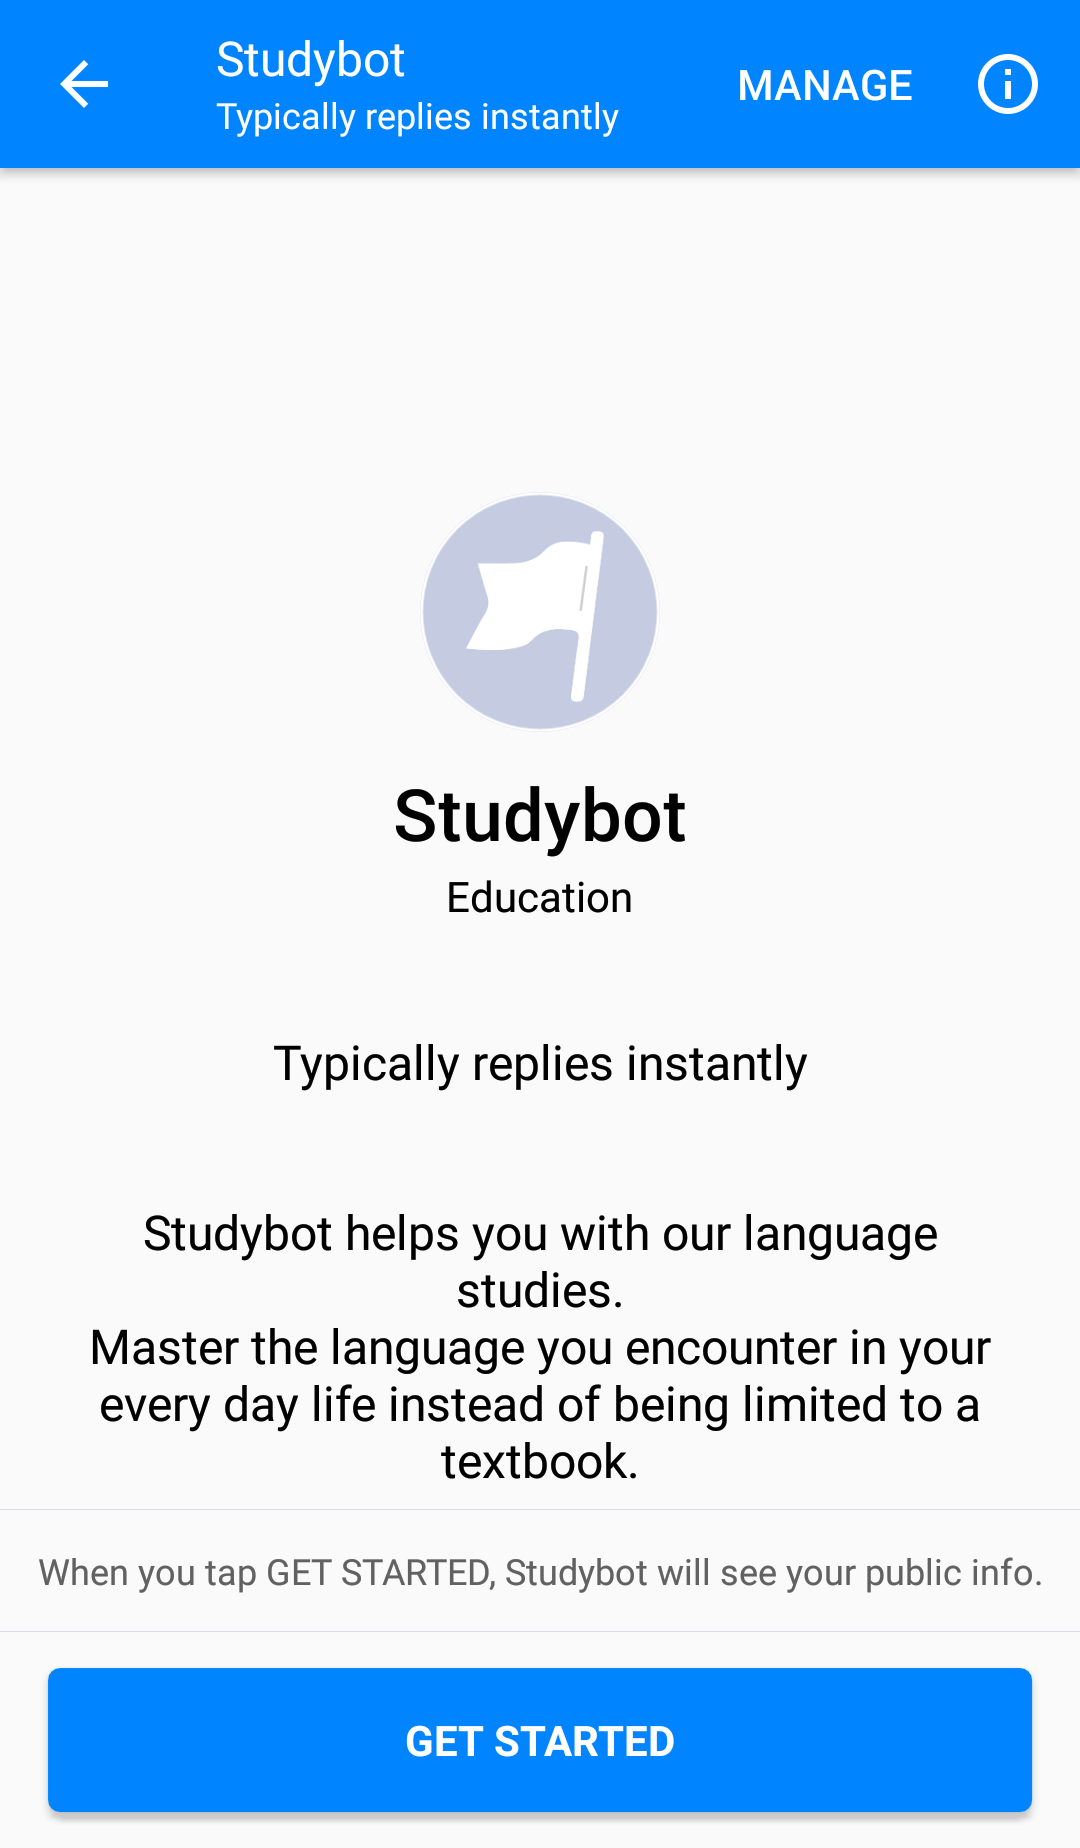
\includegraphics[width=0.28\textwidth]{images/interface/02-getstarted.png}
	\caption{Get Started Screen}
	\label{fig:02-getstarted}
\end{wrapfigure}


Before looking at the technical implementation,
the usage of the chatbot is shown from a user's point of view.
\\
The following is a presentation of the features of the chatbot
and the design of the interactions to use these features.
\\

A \emph{Facebook Page} and a \emph{Facebook Messenger bot} have been created under the name \emph{Studybot}.
\\
By not publishing the \emph{Facebook Page}, the chatbot remains only accessible for administrators of the \emph{Facebook Page}.
\\

The demonstration uses the Messenger \emph{Android} application,
but \emph{Messenger bots} can also be accesses through applications on other platforms
or using the web version of Facebook.
\\

When using the Messenger application as administrator,
the chatbot can be found by using the search as shown in figure \ref{fig:01-search}.
\\

After navigating to the chatbot,
a description becomes visible.
This can be seen in figure \ref{fig:02-getstarted}.
\\
It contains the profile image of the \emph{Facebook Page} the chatbot belongs to,
the category the \emph{Facebook Page} is part of,
and a text describing the functionality of the chatbot,
whereby all of these elements can be defined by the developer of the chatbot.
\\
A button labeled \textbf{Get Started} is displayed at the bottom of the screen.
\\

\begin{figure}[h]
  \centering
  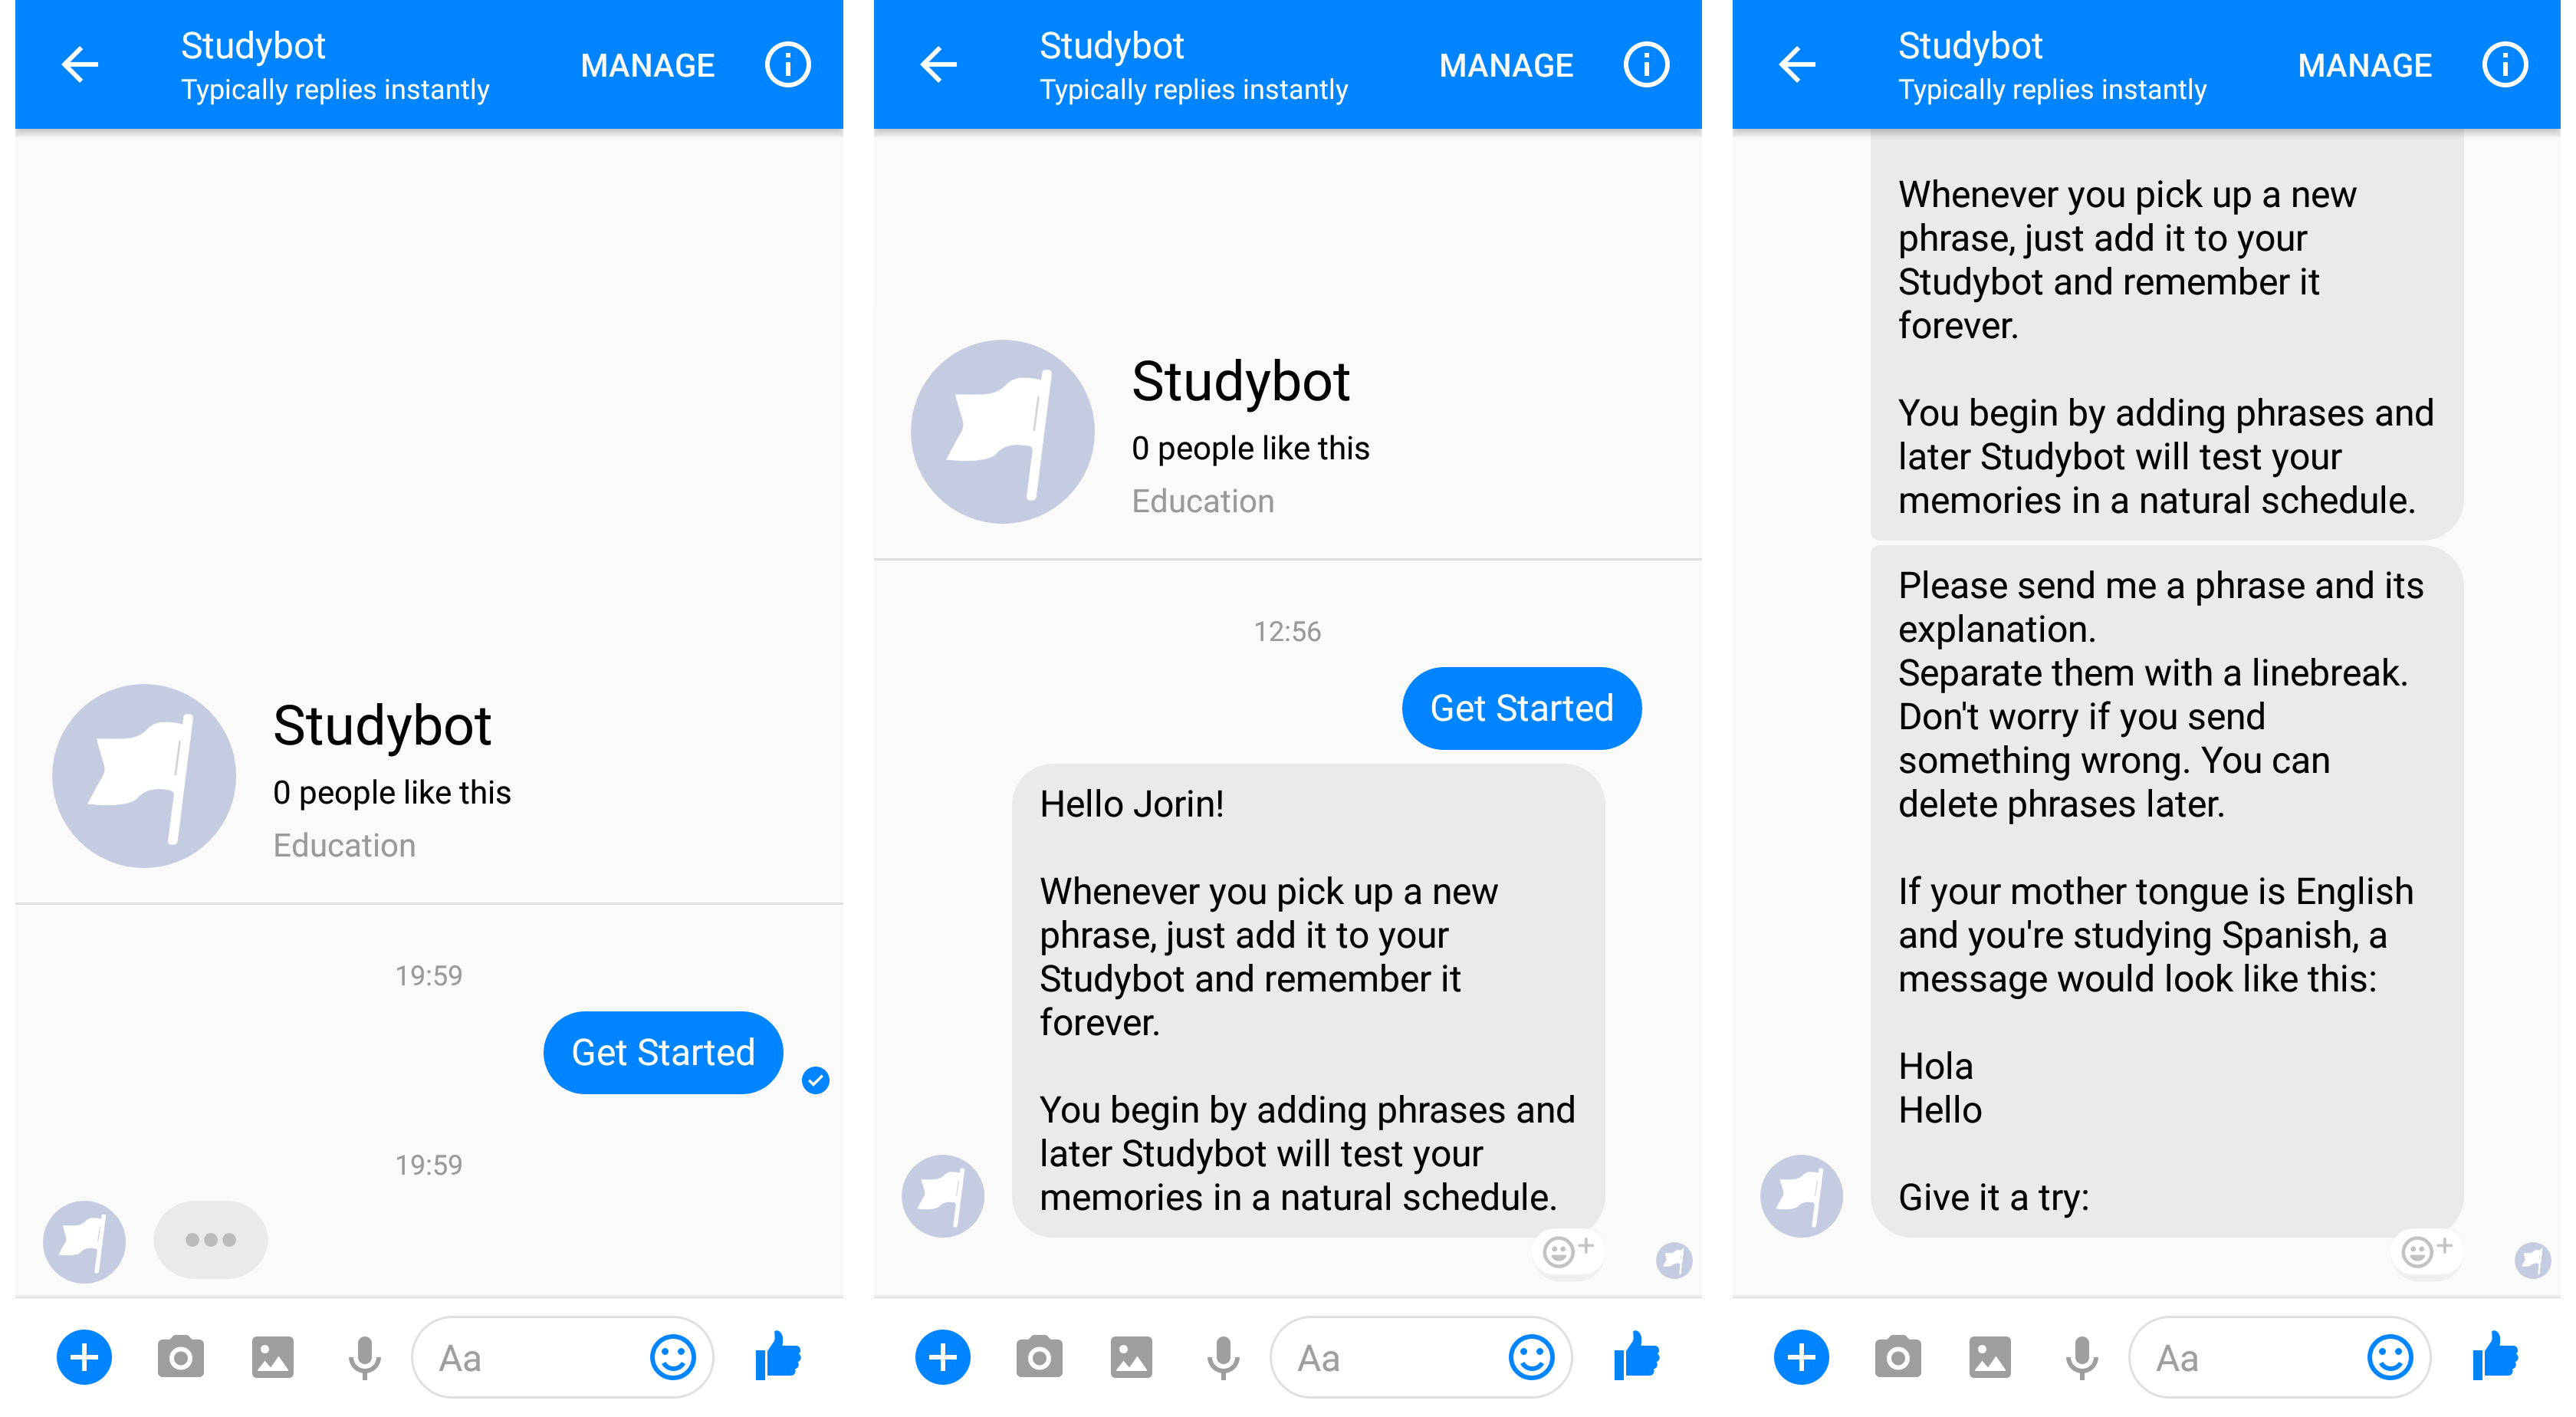
\includegraphics[width=0.9\textwidth]{images/interface/03-welcome.png}
	\caption{Introduction to Studybot}
	\label{fig:03-welcome}
\end{figure}

When pressing the \textbf{Get Started} button, a message is sent to the chatbot,
and as indicated by the \emph{dots} visible in figure \ref{fig:03-welcome} on the left image,
the chatbot is active and about to send a reply.
\\
In normal conversations the \emph{dots} are used to indicated when a user is typing.
\\
For chatbots the \emph{dots} indicate that the chatbot received the message and is crafting a reply.
\\

The image in the middle of figure \ref{fig:03-welcome} shows the first message sent to users.
They are greeted with their first name to create a more personal feeling atmosphere.
The greeting is followed by two sentences explaining the chatbot.
\\
When working with text as a medium, it is especially critical to focus on the most important information.
In graphical interfaces users can get an impression with a single glance,
but to perceive the meaning of text users need to read word by word.
\\
In most scenarios the time users are willing to invest in understanding a product is limited,
every word in a text has to be selected carefully.
\\

It can be seen in the image on the right of figure \ref{fig:03-welcome} that a second message is sent to the user.
\\
The second message is delivered 5 seconds later than the first one to not overwhelm the users with too much information at once.
\\
This message contains instructions to begin using the application.
\\
The instructions are additionally illustrated by providing an example for a message in the expected format.
\\

\begin{figure}[h]
  \centering
  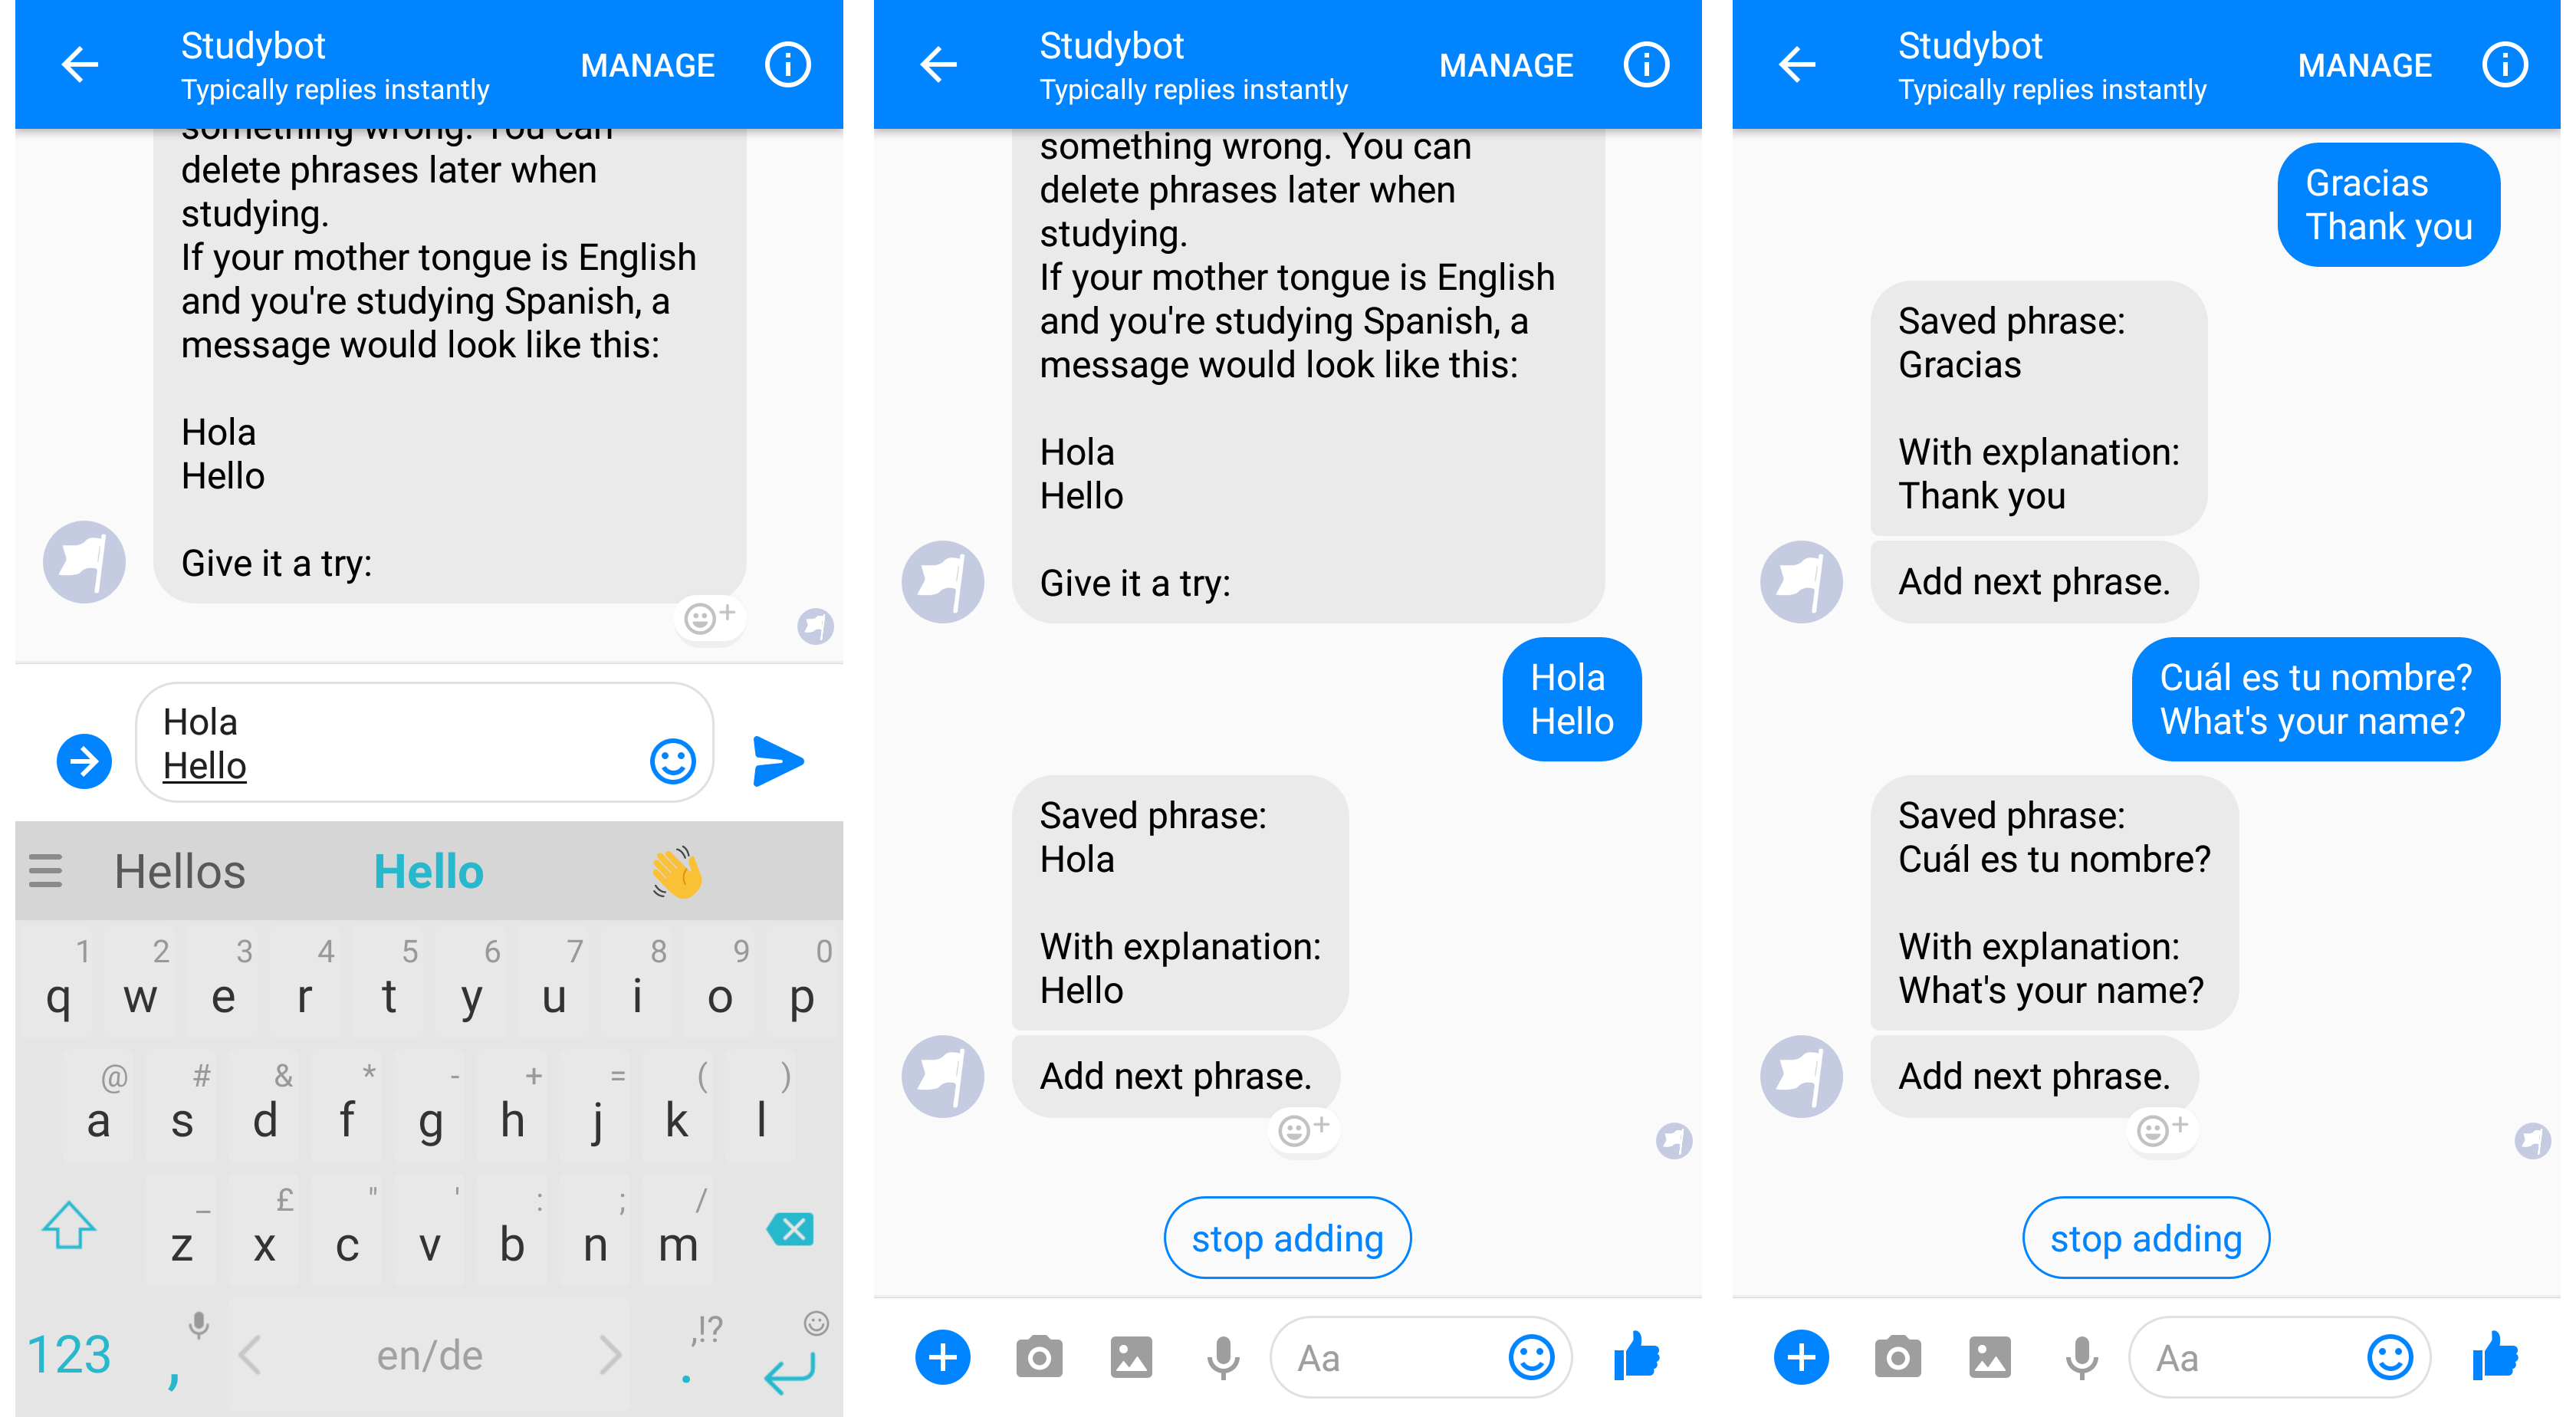
\includegraphics[width=0.9\textwidth]{images/interface/04-add.png}
	\caption{Adding three phrases}
	\label{fig:04-add}
\end{figure}

At this point the user needs to interact with the chatbot.
\\
Figure \ref{fig:04-add} shows how a user adds phrases to \emph{Studybot}.
When typing a phrase, users first type the phrase in the foreign language they like to study,
then a \emph{line-break} needs to be added,
and the next line contains an explanation for the preceding phrase.
\\
After the phrase is sent to the chatbot,
a confirmation message is displayed to keep the user updated about the current state of the system.
\\
This is followed by another message prompting the user to add more words.
\\

\begin{wrapfigure}{O}{0.3\textwidth}
  \centering
  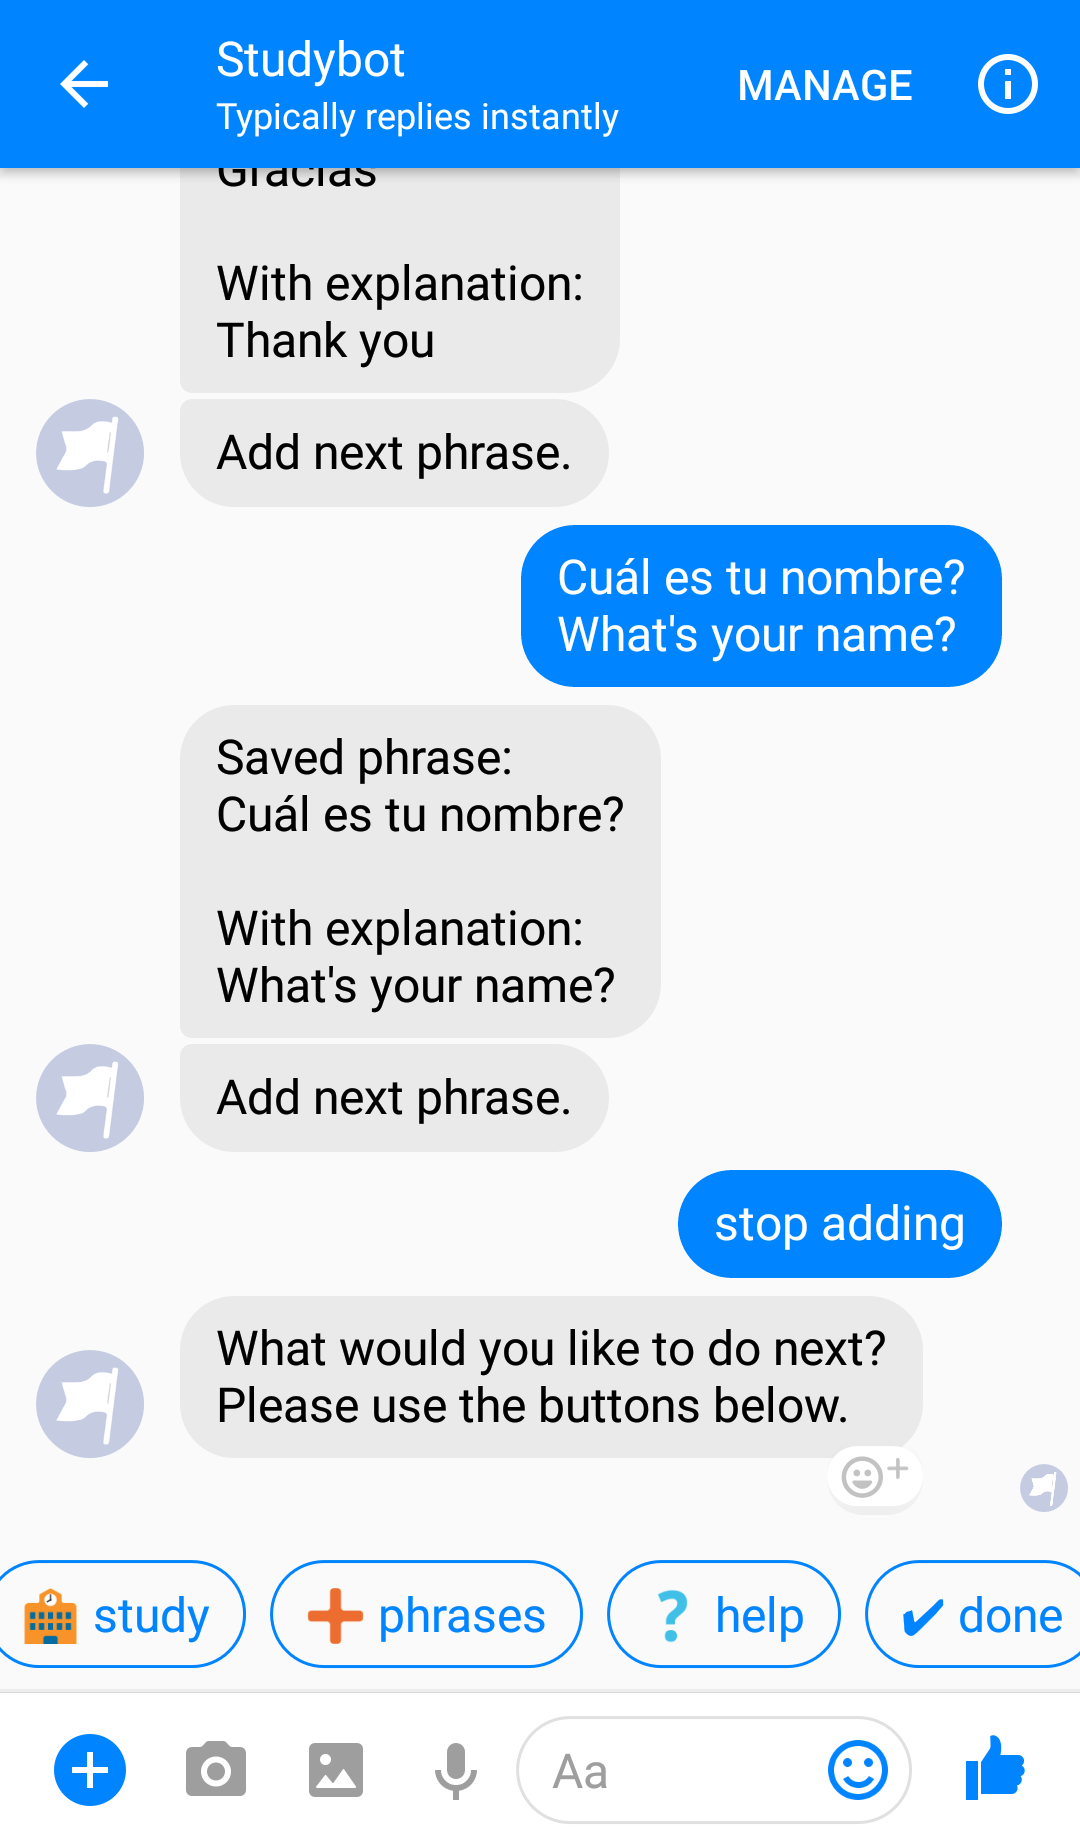
\includegraphics[width=0.28\textwidth]{images/interface/05-stop-adding.png}
	\caption{Stop adding phrases}
	\label{fig:05-stop-adding}
\end{wrapfigure}

For a chatbot it is critical to always keep the user informed about the next expected action,
therefore most messages should end with a prompt for the next input.
\\

The image in the middle of figure \ref{fig:04-add} has a button displayed at the bottom of the messages,
which the user can use as an alternative way for interacting with the chatbot.
\\

As shown in figure \ref{fig:04-add}, three phrases have been added to \emph{Studybot}
before the user decides to press the button labeled as \textbf{stop adding}.
\\
Figure \ref{fig:05-stop-adding} shows, that after stopping the adding of phrases, the user is prompted with an array of four possible actions.
The actions are labeled as \textbf{study}, \textbf{+ phrases}, \textbf{help} and \textbf{done}.
Each button label also contains an emoji\footnote{``Emoji are pictographs (pictorial symbols) that are typically presented in a colorful form and used inline in text. They represent things such as faces, weather, vehicles and buildings, food and drink, animals and plants, or icons that represent emotions, feelings, or activities.''~\cite{emoji}} used as icon for the action to make it easier identifiable for users.
\\
When the usage of graphical elements is limited and one has to rely mainly on text for communication,
emojis can be a helpful substitution for traditional icons to provide visual guidance.
\\

The chatbot has different \emph{modes} of interaction.
\\
Internally the chatbot needs to keep track of the current \emph{mode} of each user to be able
to address each message in the correct context.
\\
In figure \ref{fig:05-stop-adding} the user has left the \emph{mode} for adding words
and entered the \emph{menu mode} which provides access to other modes.
\\

\begin{figure}[h]
  \centering
  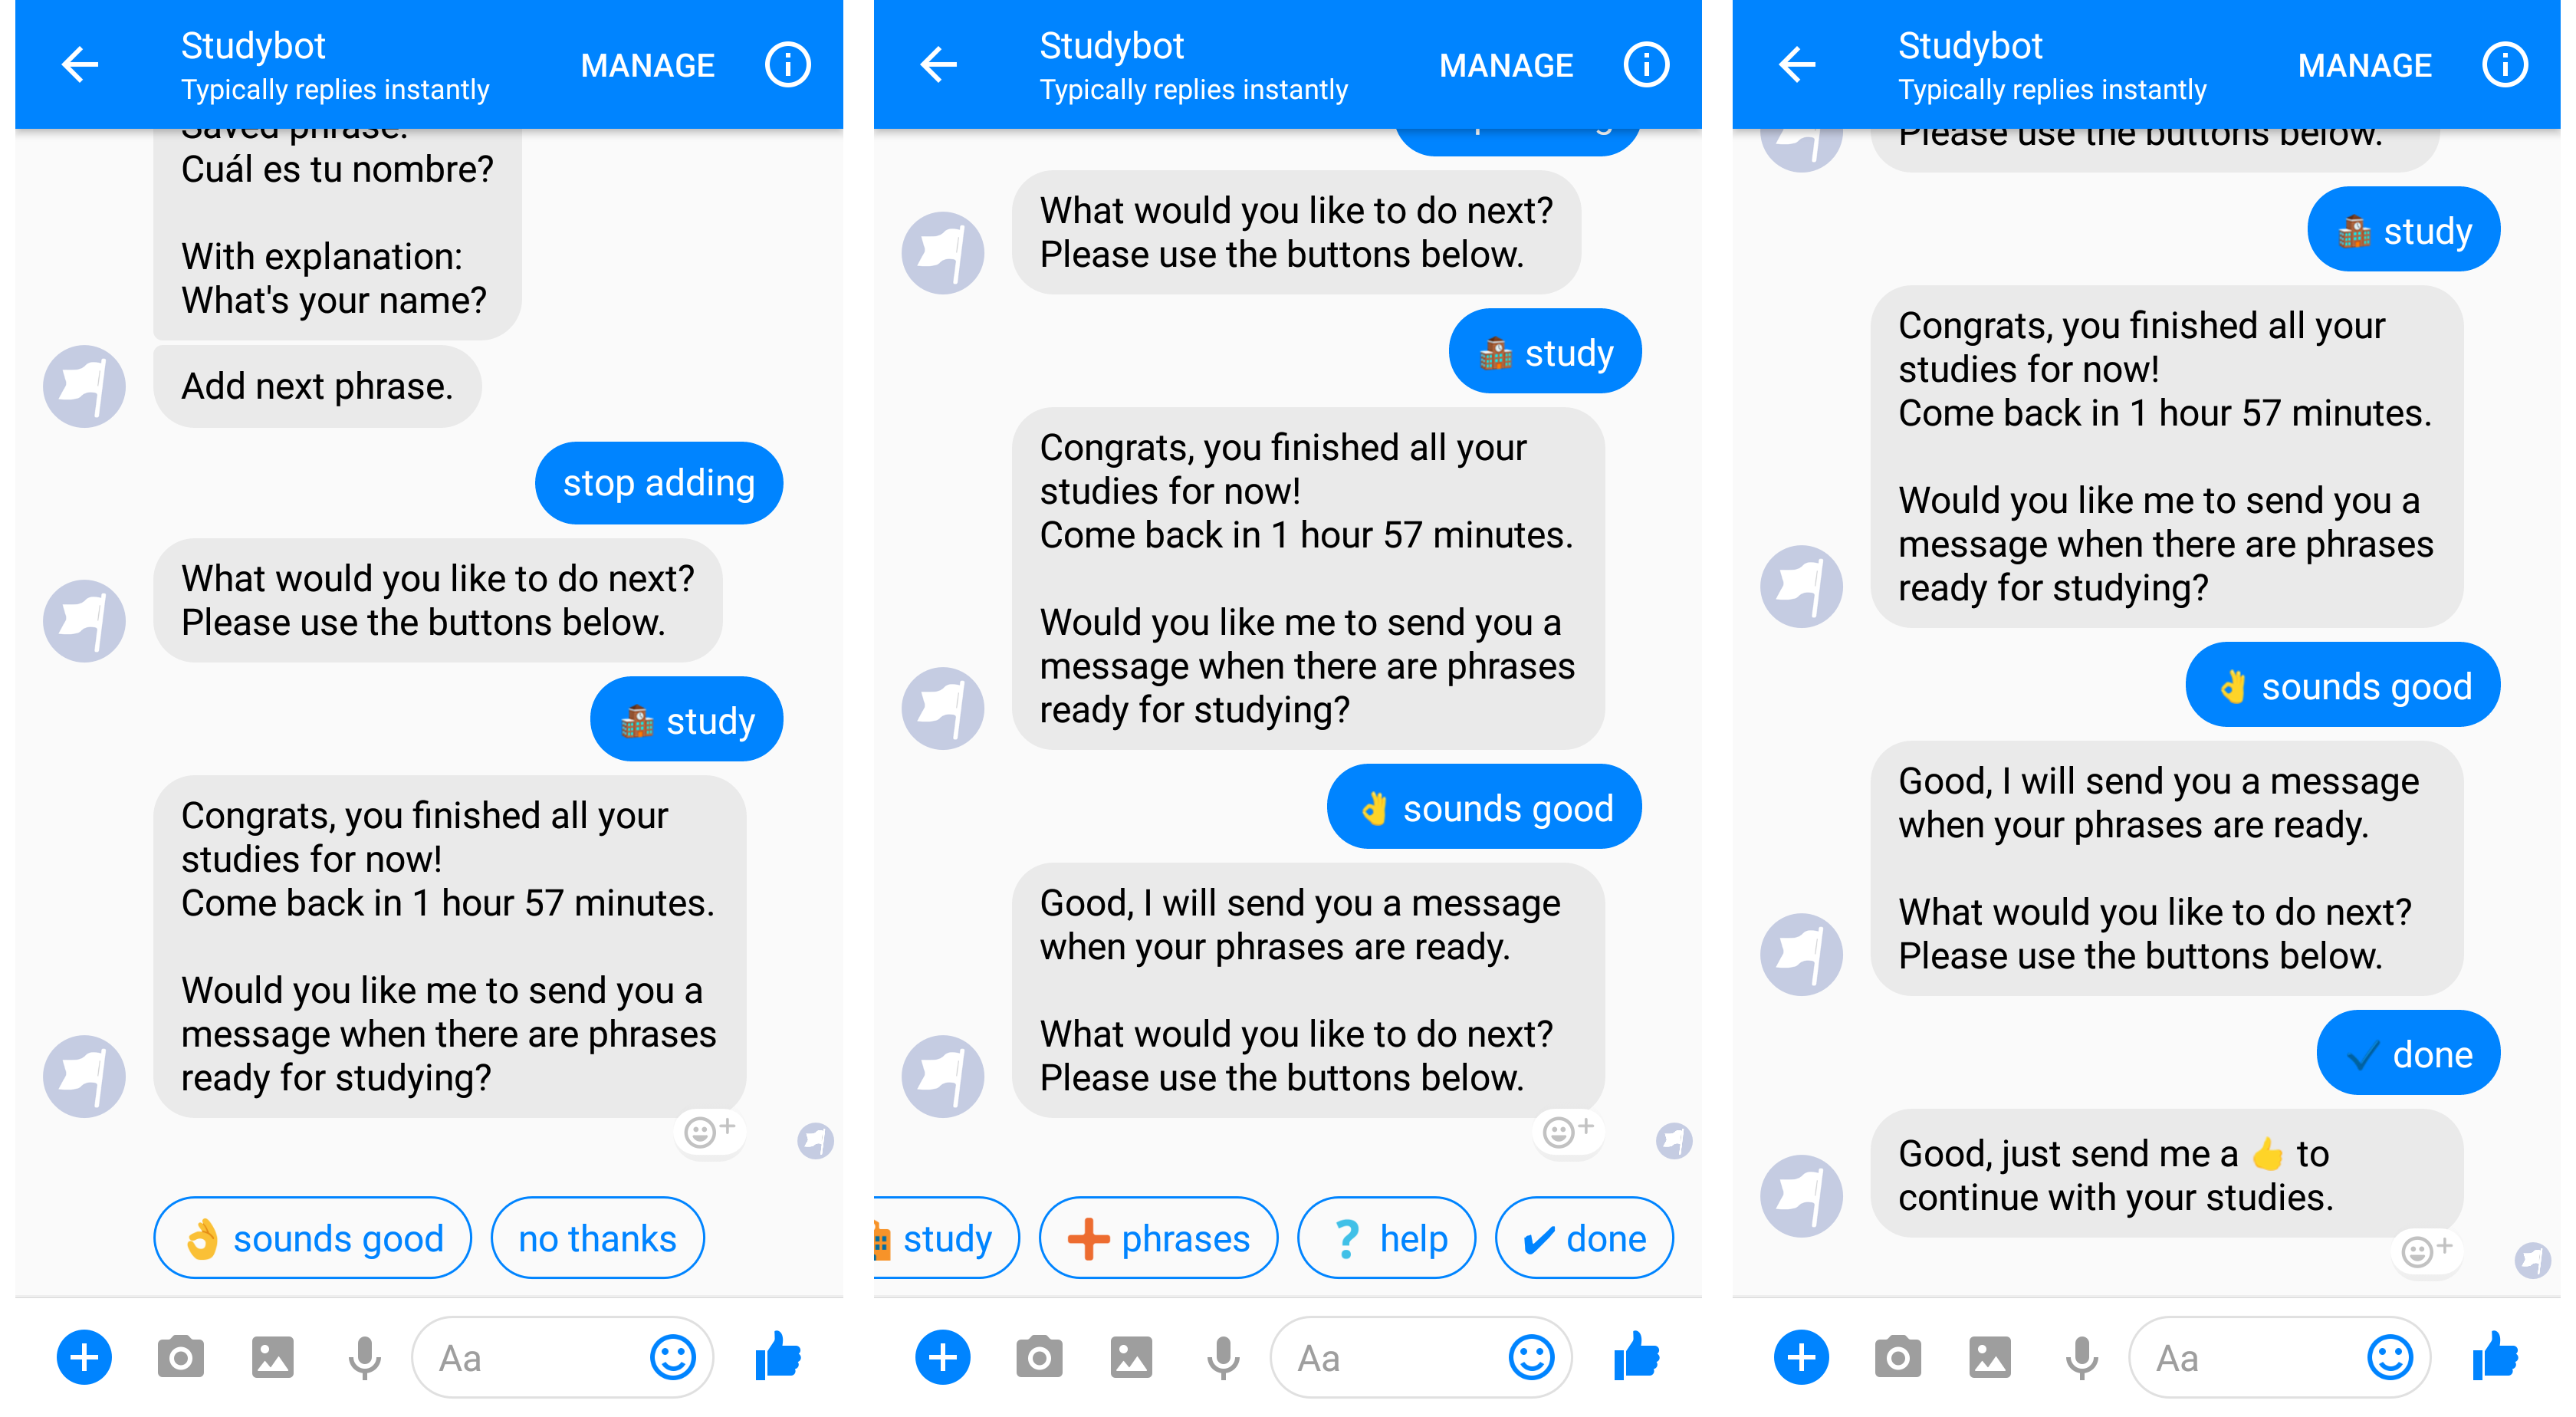
\includegraphics[width=0.9\textwidth]{images/interface/06-enable-notify.png}
	\caption{Attempt to study and activation of notifications}
	\label{fig:06-enable-notify}
\end{figure}

By clicking on the button labeled \textbf{study},
the user switches to the \emph{mode} for studying of the added vocabulary.
\\
However, as the image on the left of figure \ref{fig:06-enable-notify} shows,
the added phrases cannot be studied yet.
\\

\emph{Studybot} uses a concept known as \emph{spaced repetition system}, or short \emph{SRS},
which makes use of the so called \emph{spacing effect}. ``Information that is spaced over time is better remembered than the same amount of information massed together''~\cite{srs}.
\\
Based on this approach users need to wait before studying newly added vocabulary.
The more often a phrase is guessed correctly the less frequent the user will be asked to review the phrase.
\\

\begin{figure}[h]
  \centering
  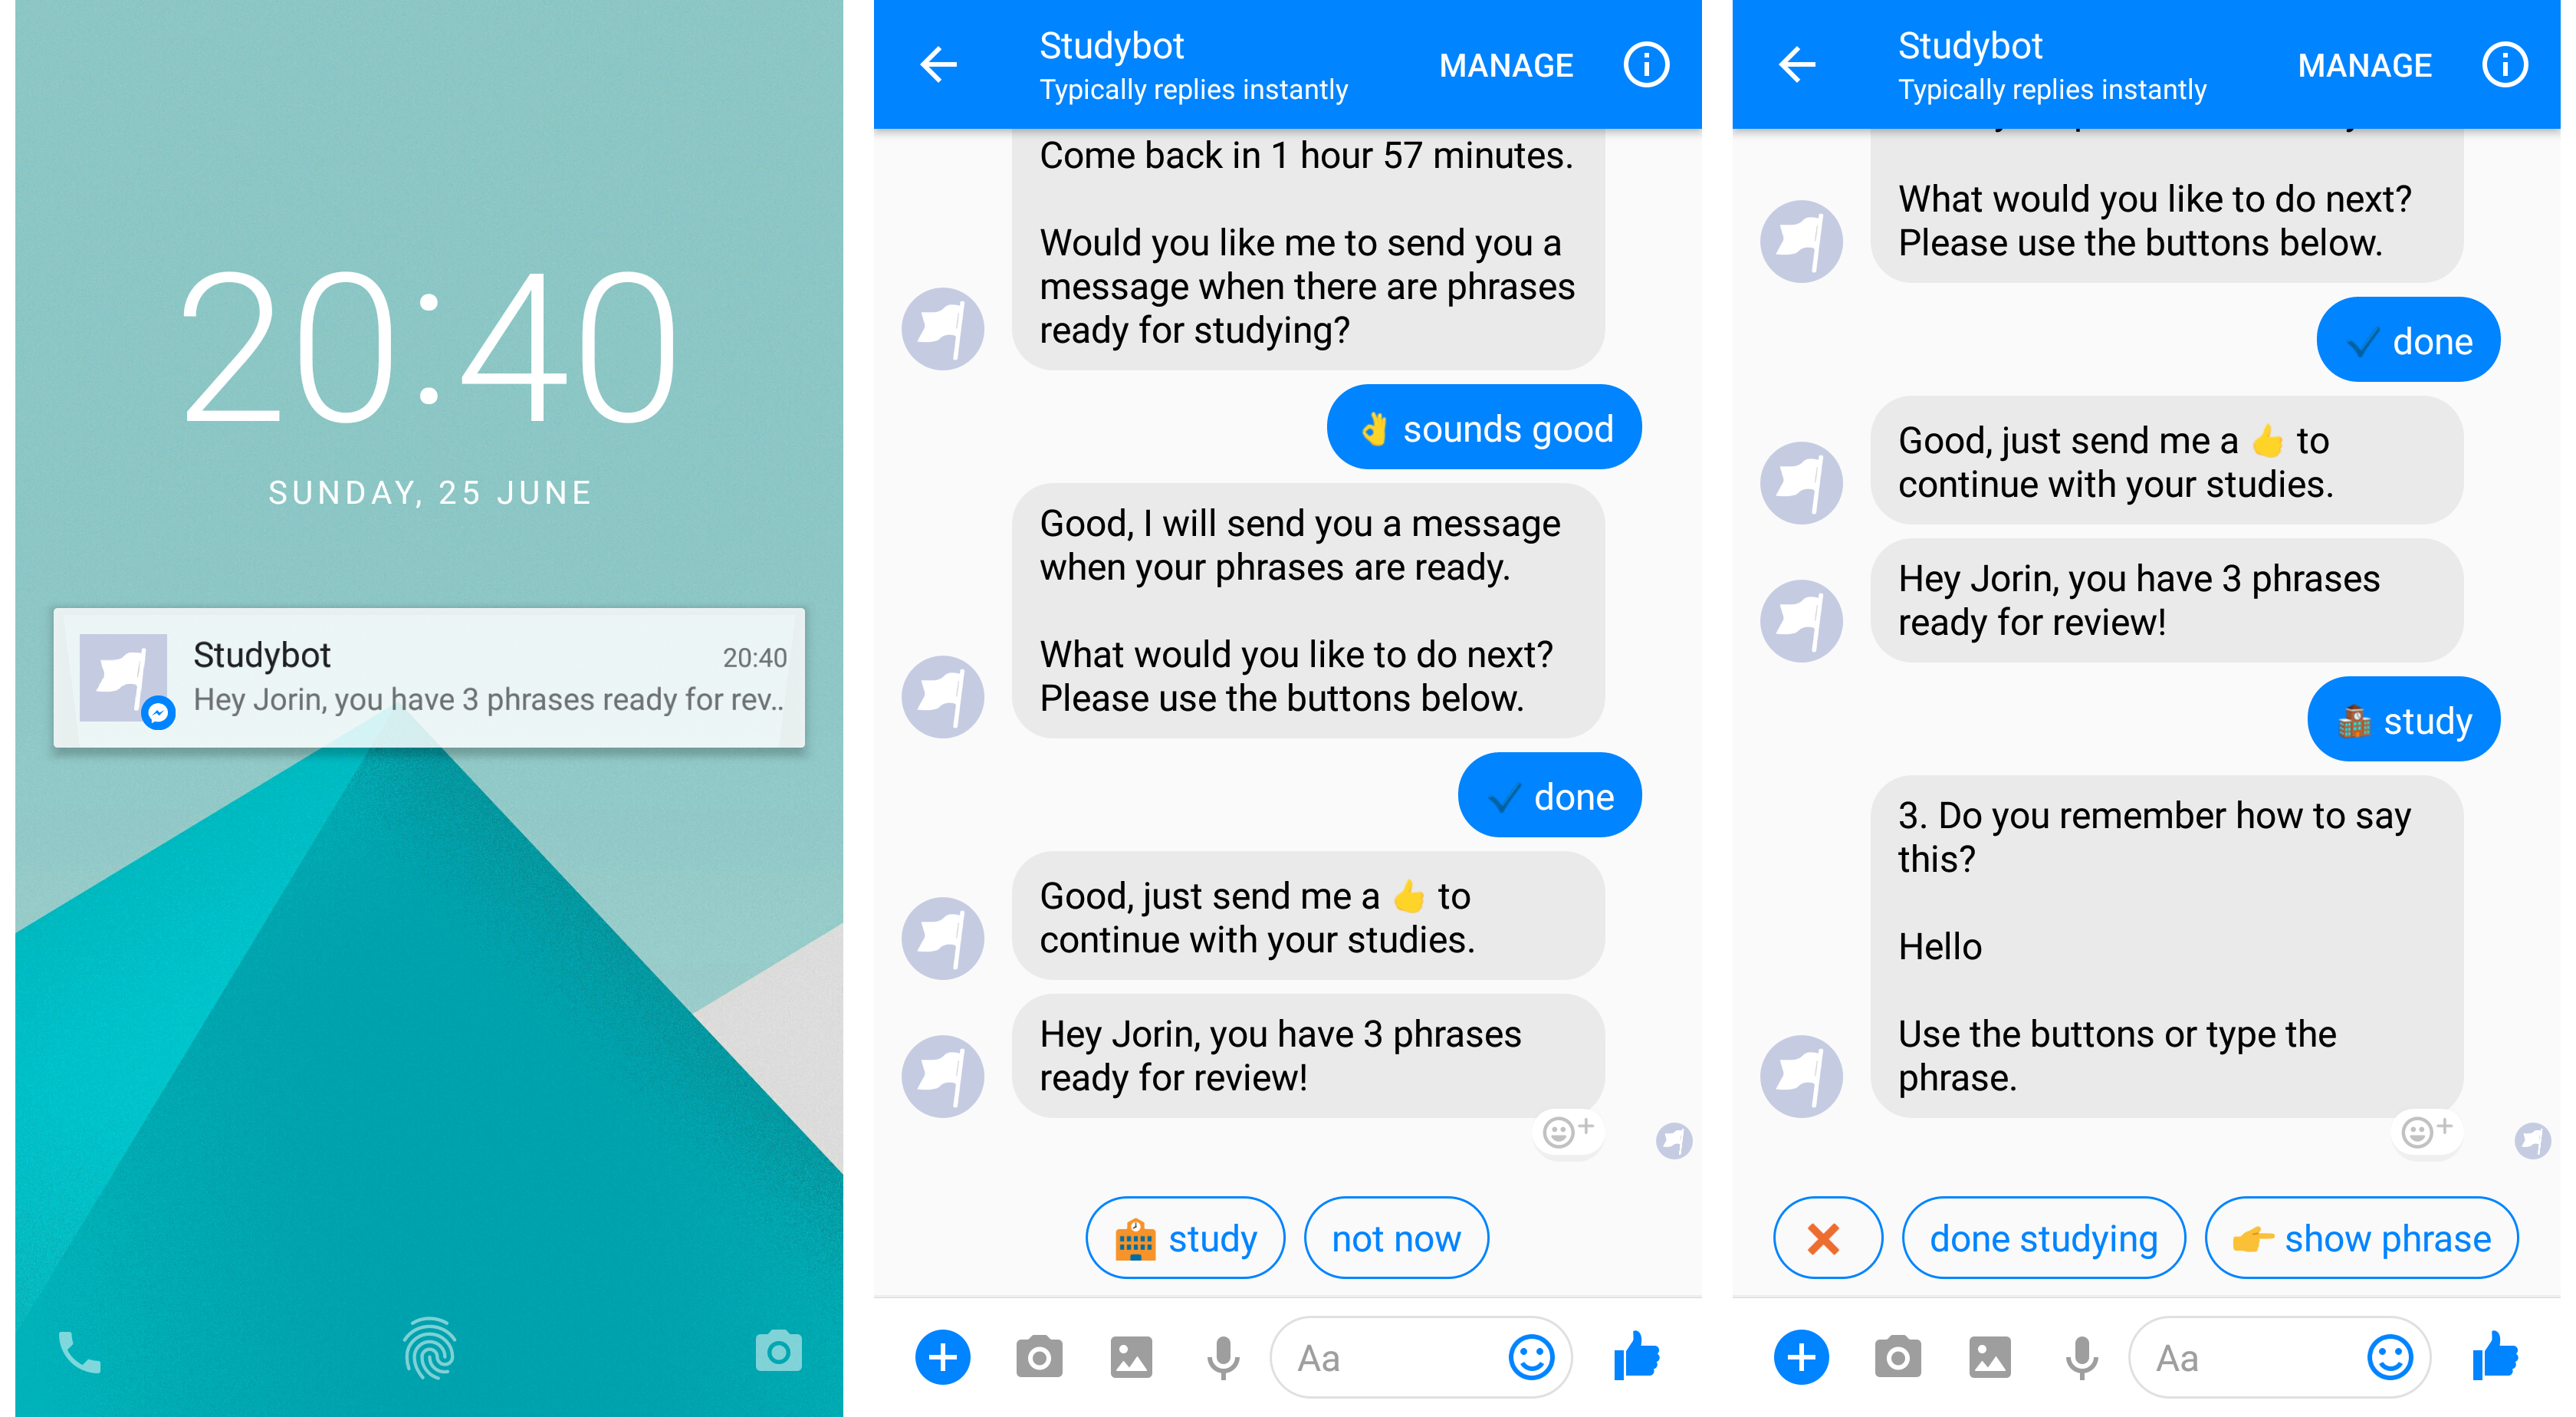
\includegraphics[width=0.9\textwidth]{images/interface/07-notify-study.png}
	\caption{Notification message and beginning of study}
	\label{fig:07-notify-study}
\end{figure}

Since added phrases can not be studied directly,
the user is instead offered to receive a notification message once phrases are ready for review.
\\

When sending notifications to users, it is crucial to not send more messages than necessary.
\\
Depending on the messenger platform, there are also policies in place on how many messages are permitted.
\\
The platform policy of \emph{Facebook Messenger} clearly requires to
``respect all requests (either on Messenger or off) by people to block, discontinue, or otherwise opt-out of your using Messenger to communicate with them''~\cite{fbpolicy},
which means that there needs to be a way for users to disable the sending of notifications.
Further the platform policy clarifies that ``you may message people within 24 hours of a person's interaction with your business or Bot ..., and until the next interaction, you may send one additional message after this 24 hour period in order to follow up on your conversation''~\cite{fbpolicy}.
\\
How notifications can be disabled in \emph{Studybot} is not further explained here,
but an illustration of the feature can be found in the appendix in figure \ref{fig:10-disable-notify} on page \pageref{fig:10-disable-notify}.
\\

\begin{figure}[h]
  \centering
  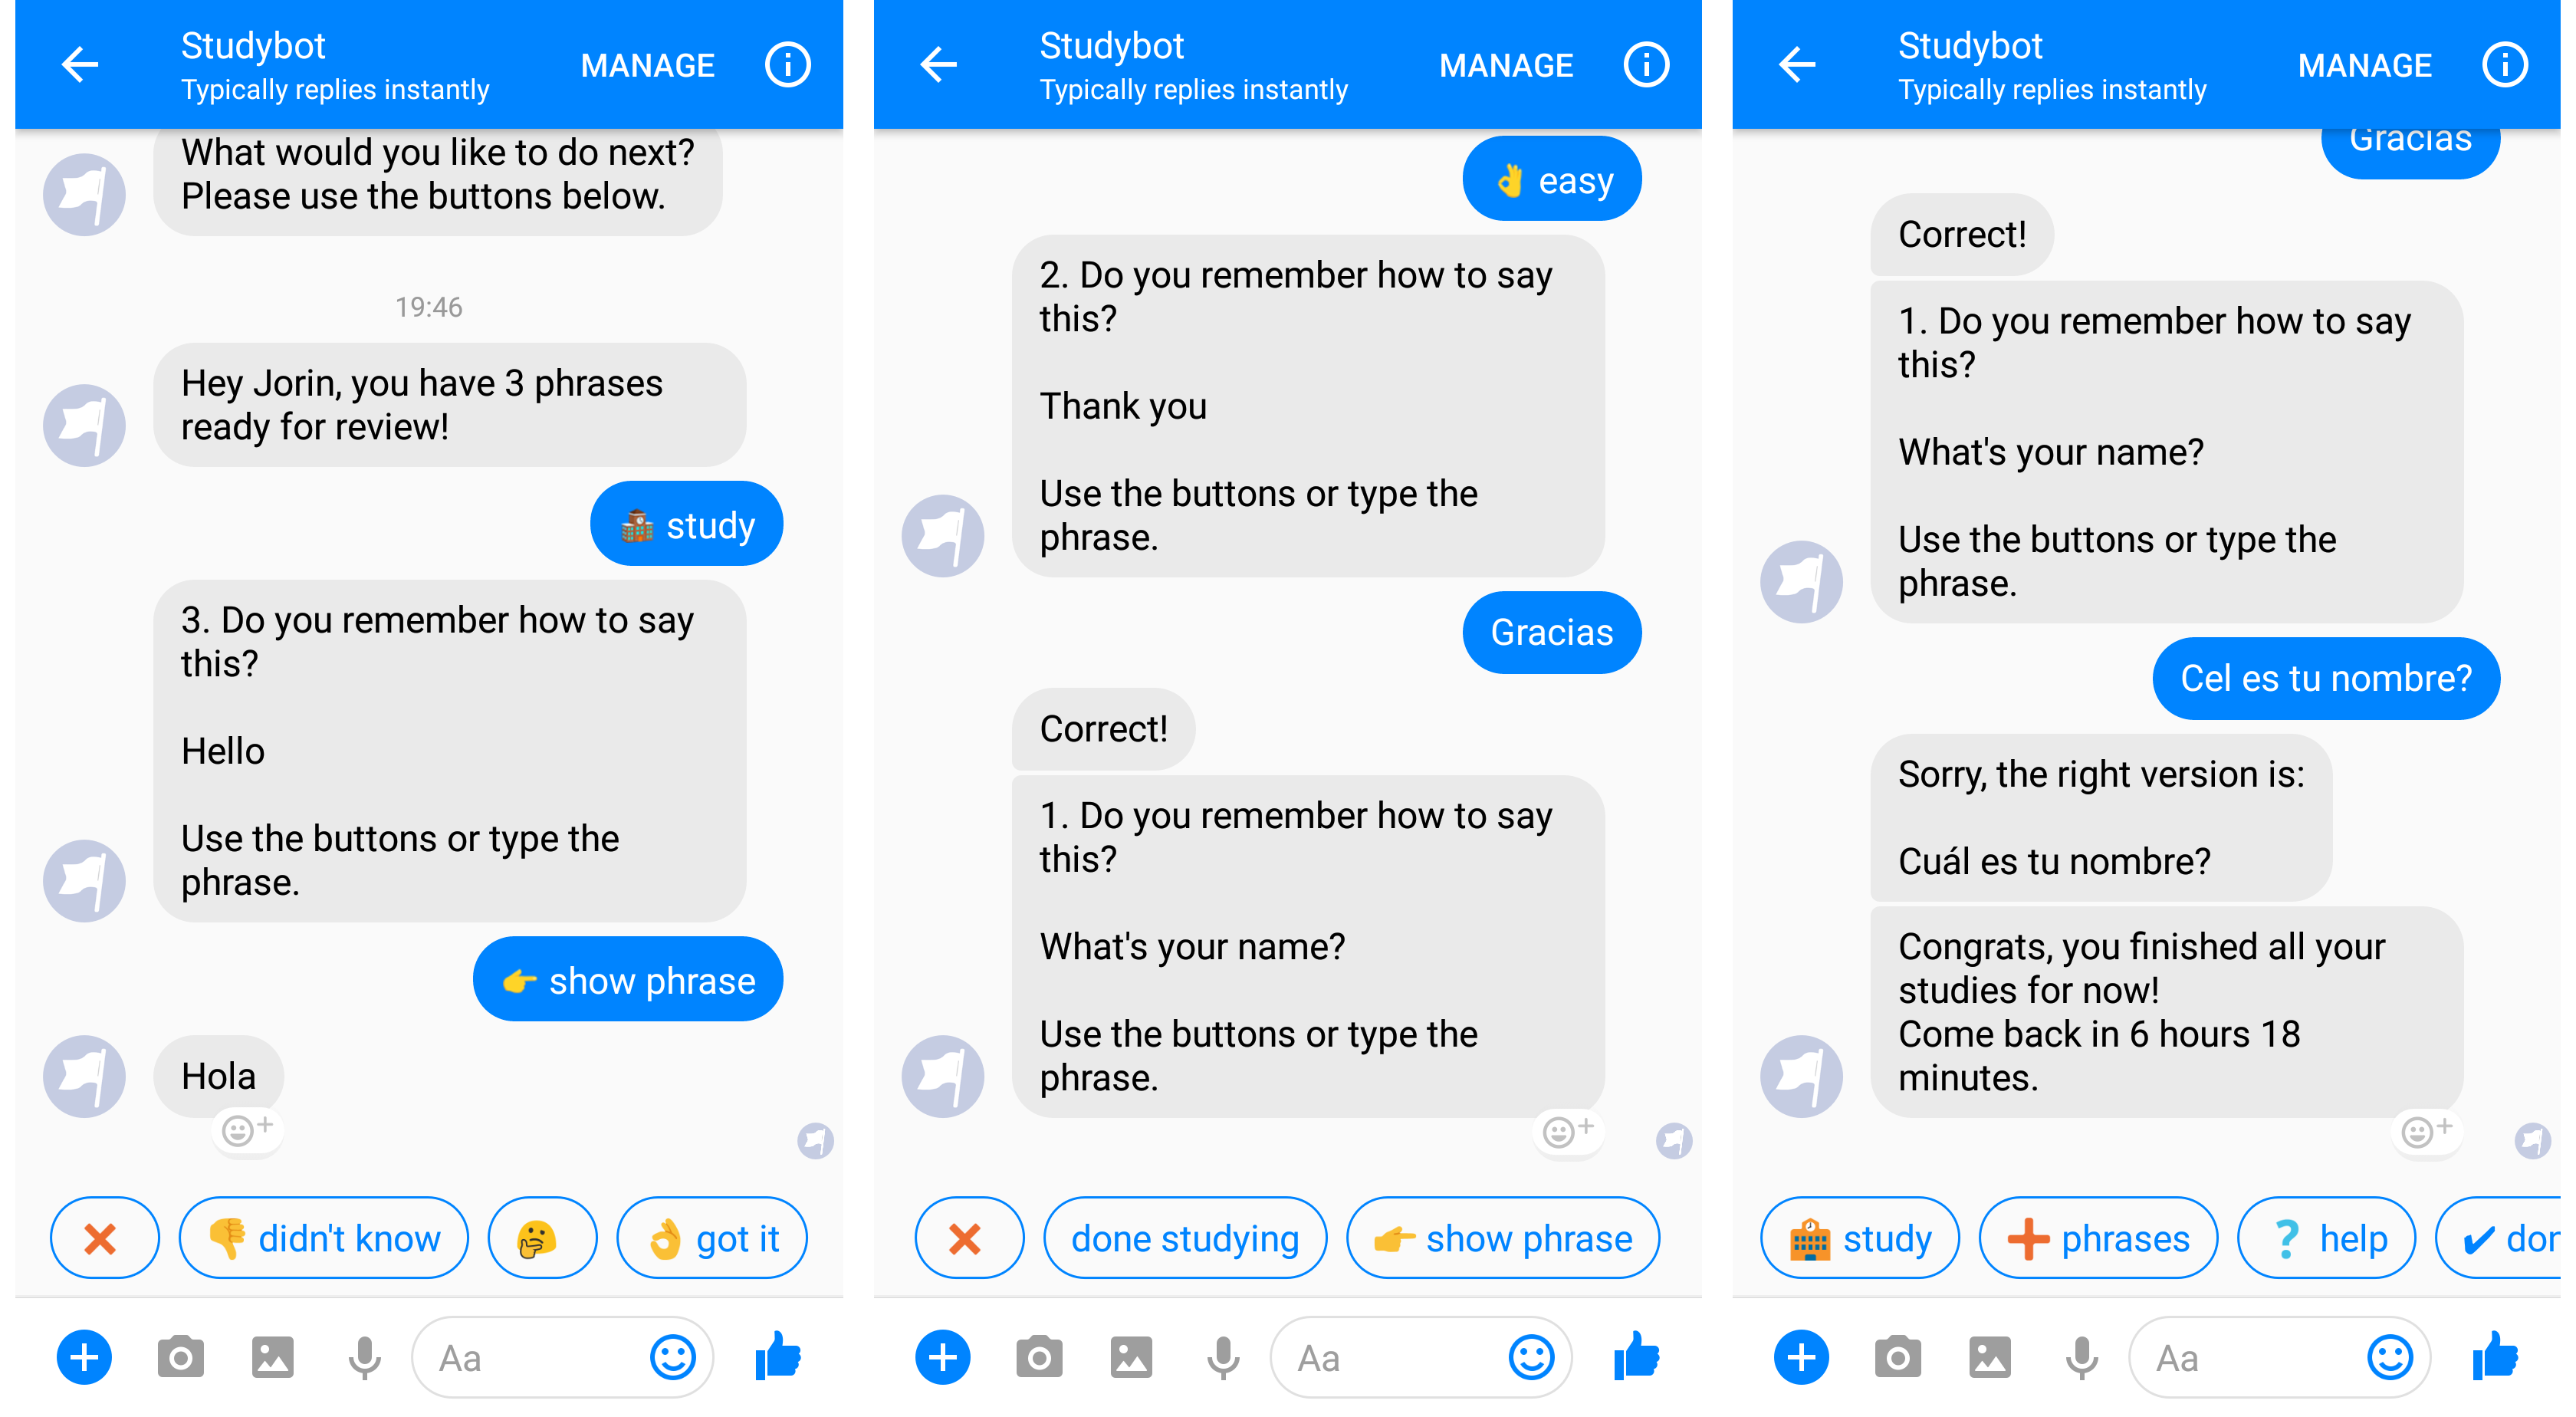
\includegraphics[width=0.9\textwidth]{images/interface/08-study-done.png}
	\caption{Study using buttons or by typing}
	\label{fig:08-study-done}
\end{figure}

In figure \ref{fig:07-notify-study} a notification from the \emph{Messenger} application is shown on the mobile phone.
\\
It is triggered when enough studies are ready to be reviewed.
\\
When opening the conversation with the chatbot,
the user is now prompted to study.
\\
As defined as a requirement in \ref{funcreq} on page \pageref{funcreq},
while studying one is free to choose to answer either by using the buttons at the bottom of the screen
or by directly typing the correct phrase.
\\

The \textbf{x} button available on the right image of figure \ref{fig:07-notify-study},
allows users to delete a phrase.
\\
Since there is no possibility in \emph{Facebook Messenger} to display a long list of interactive elements to the user,
creating separate functionality for editing and deleting phrases is difficult to achieve,
and during studying is the only possible moment to refer to a phrase.
\\

The figures \ref{fig:07-notify-study} and \ref{fig:08-study-done} show a subtle decision to display the buttons users are most likely to interact with
on the right side.
\\
Since the English language is written from left to right and we scan text accordingly,
it is more intuitive to show the most important information on the left,
however certain interactions, like studying, need to be performed so frequently,
that a user will remember the location of the buttons quickly and does not need to \emph{scan} the interface every single time.
\\
In this scenario it is helpful to have the most used action on the right side, because the majority of humans are right-handed \cite{righthand},
and they can therefore reach the buttons on the right with less effort since they are closer to the thumb when using a mobile phone single-handed.
\\

\begin{figure}[h]
  \centering
  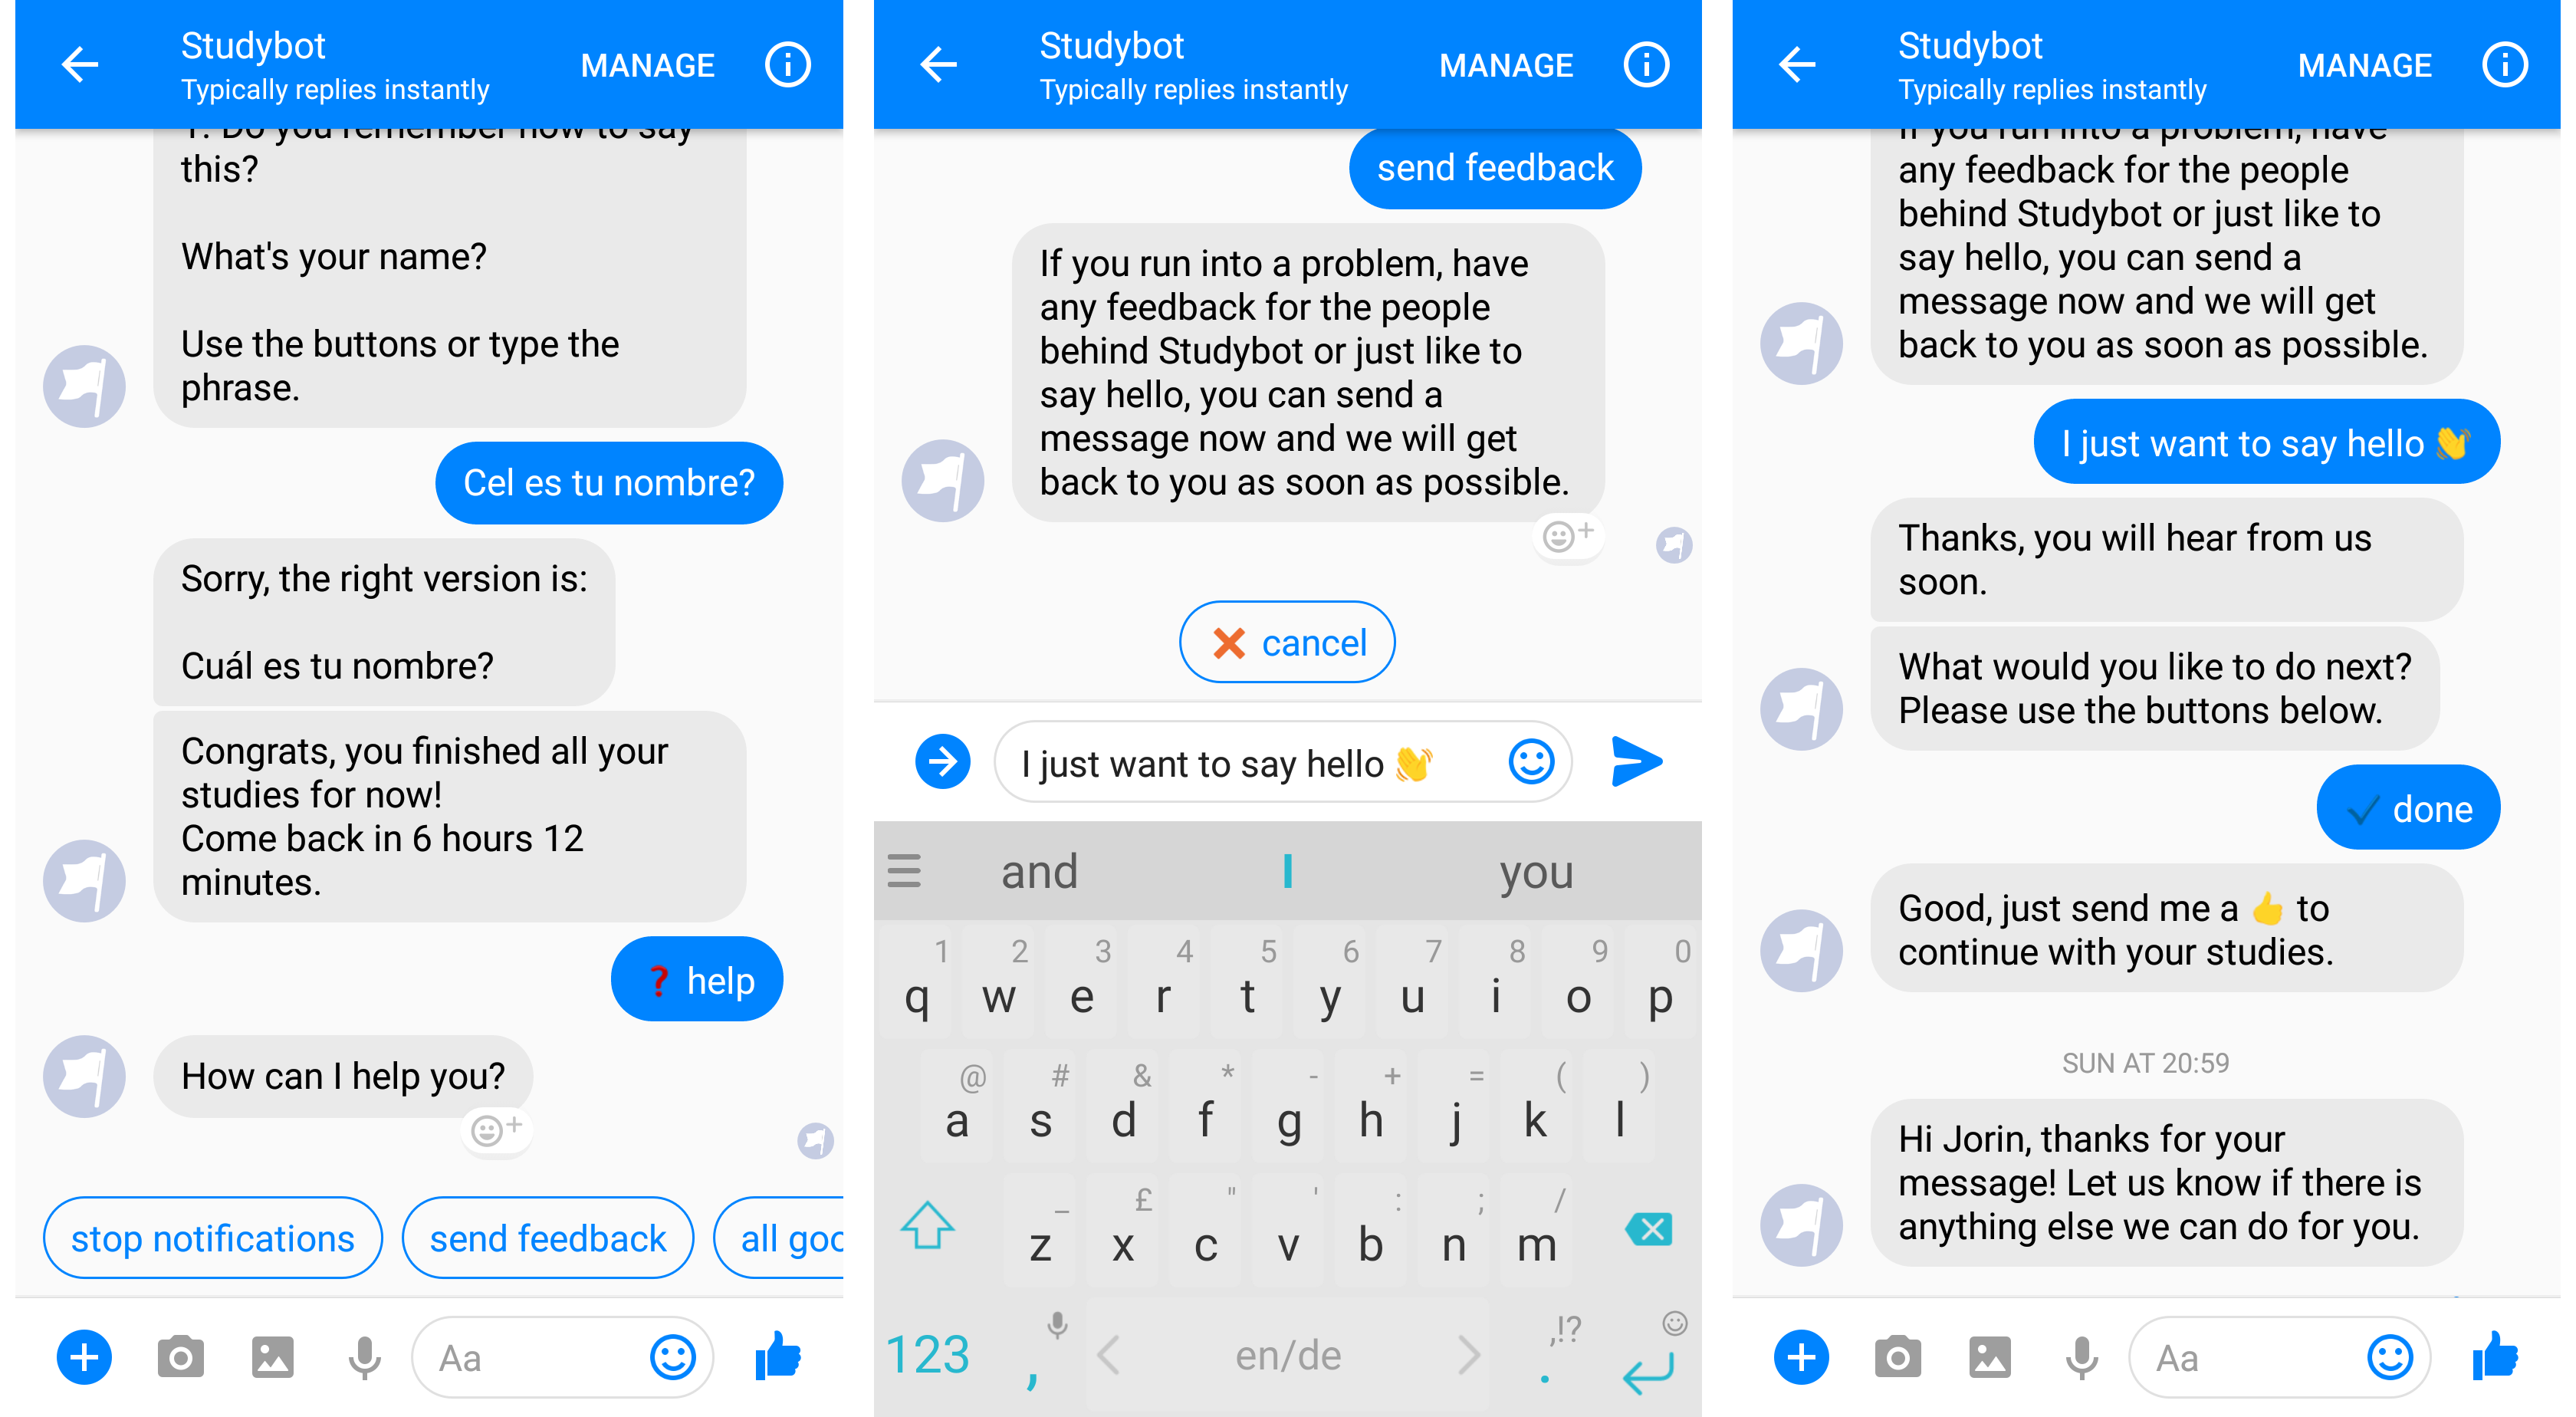
\includegraphics[width=0.9\textwidth]{images/interface/09-feedback.png}
	\caption{Send feedback and receive a reply}
	\label{fig:09-feedback}
\end{figure}

\label{slackhook}

A feature, that is outside of the main flow of \emph{Studybot}, is the sending of feedback to the developers of the chatbot.
\\
As shown in figure \ref{fig:09-feedback}, it can be accessed after pressing the \emph{help} button.
\\
This feature is not specific to language studying and it is useful for most chatbots.
\\
Normally all messages are answered automatically by the chatbot,
but there should be a way for users to talk to the human developers or administrators that provide the chatbot.
\\
The feature is automated by sending the messages that users send as \emph{feedback}
to a \emph{Slack channel}~\cite{slack}.
\\
Additionally administrators can directly reply to user messages inside \emph{Slack}
and the replies are send back to the correct users within the chatbot.
\\
Figure \ref{fig:09-feedback} shows the flow for sending feedback from a user's point of view.
\\
The exact implementation is hidden from users,
but simplifying the sending of replies by using an existing medium like \emph{Slack},
can minimize the manual work required to maintain a personal feature like this.
\\


All primary interactions the example chatbot provides have been covered above.
\\
Many of the implemented interactions can be transfered and reused when creating other kinds of chatbots;
addressing users by name,
sending text in small chunks with a delay in between,
prompting users for specific input with every message,
keeping track of the context of each user,
asking for permission before sending notifications,
consciously ordering buttons and
supporting custom user feedback,
these patterns can be applied in many different scenarios.
\\

The resulting functionality and implementation of the example chatbot can be summarized as finding the simplest possible interaction for the user to get a task done, which is expressed well in the following quote from the newspaper \emph{The Guardian}~\cite{digiday} about the lessons they learned by developing a chatbot:

\begin{quote}
A lot of users responded as they would to a human, and when they got non-human responses, they’d stop using it, said Wilk. So the Guardian went in the opposite direction with its news bot and aimed for utter simplicity. The lesson, according to Wilk, was: “Don’t build people’s expectations too much of what’s possible, just keep it simple.”
\end{quote}
